\documentclass[a4paper, 12pt]{beamer}

\usetheme{metropolis}
% Paquetes necesarios
\usepackage[utf8]{inputenc}
\usepackage[T1]{fontenc}
\usepackage{helvet}
\usepackage[spanish]{babel}
\usepackage{amsmath, amssymb, amsfonts, amsthm, amssymb}
\usepackage{cite}
\usepackage{listings}
\usepackage{color}
\usepackage{graphicx}
% Información del título
\title{\textcolor{cyan}{Moogle!}}
\subtitle{Proyecto de Programación I: Buscador inteligente.}
\author{Melissa Maureen Sales Brito}
\institute{MatCom}
\date{}

% Contenido de la presentación
\begin{document}

\maketitle

\begin{frame}{\textcolor{cyan}{Índice}}
\tableofcontents
\end{frame}

\section{Introducción}

\subsection{Definición general}
\begin{frame}{\textcolor{cyan}{Introducción}}
Moogle! es una aplicación totalmente original cuyo propósito es buscar inteligentemente un texto en un conjunto de documentos.


Es una aplicación web, desarrollada con tecnología .NET Core 6.0, específicamente usando Blazor como {\it framework} web para la interfaz gráfica, y en el lenguaje {\tt C\#}. 
\end{frame}

\subsection{Componentes, requisitos e instrucciones}

\begin{frame}{\textcolor{cyan}{Componentes, requisitos e instrucciones}}
    La aplicación está dvidida en dos componentes fundamentales:
    \begin{itemize}
        \item {\tt MoogleServer} es un servidor web que renderiza la interfaz gráfica y sirve los resultados.
        \item {\tt MoogleEngine} es una biblioteca de clases donde está implementada la lógica del algoritmo de búsqueda.     
    \end{itemize}
\end{frame}

\begin{frame}{\textcolor{cyan}{Componentes, requisitos e instrucciones}}
    Necesitas tener instaldo algún navegador y tener a {\tt dotnet} disponible, o equivalente a esto tener .NET CORE 6.0 instalado, para 
    ejecutarlo te debes ubicar en la carpeta del proyecto y ejecutar en la terminal de Linux:
     {\tt make dev}
    
     Si estás en Windows, debes poder hacer lo mismo desde la terminal del WSL (Windows Subsystem for Linux), el comando ultimate para ejecutar la aplicación es (desde la carpeta raíz del proyecto):
    {\tt dotnet watch run --project MoogleServer}
    \begin{itemize}
        \item Abrir en el navegador {\tt localhost:5000/}
        \item Introducir la b\'usqueda en la ``entrada'' y presionar el bot\'on {\tt ``Buscar''}
    \end{itemize}
\end{frame}

\begin{frame}{\textcolor{cyan}{Componentes, requisitos e instrucciones}}
    \begin{itemize}
        \item {\small En primer lugar, el usuario puede buscar no solo una palabra sino en general una frase cualquiera.}
        \item {\small Si no aparecen todas las palabras de la frase en un documento, pero al menos aparecen algunas, este documento también será devuelto, pero con un score menor mientras menos palabras aparezcan.}
        \item {\small Algunas palabras excesivamente comunes como las preposiciones, conjunciones, etc., serán ignoradas por completo ya que aparecerán en la inmensa mayoría de los documentos. (En este sentido se recomienda un content de archivos en un mismo idioma.)}
    \end{itemize}
\end{frame}

\begin{frame}{\textcolor{cyan}{Componentes, requisitos e instrucciones}}
    
    {\tt Nota:} el uso de los siguientes operadores debe ser igual al de los ejemplos, para cada palabra que se desee negar/fijar/priorizar.
    \begin{itemize}
        \item {\small Un símbolo $!$ delante de una palabra (e.j., hardin $!$tessa) indica que esa palabra no debe aparecer en ningún documento que sea devuelto.}
        \item {\small Un símbolo \textasciicircum delante de una palabra (e.j., hardin \textasciicircum tessa) indica que esa palabra tiene que aparecer en cualquier documento que sea devuelto.}
    \end{itemize}
\end{frame}

\begin{frame}{\textcolor{cyan}{Componentes, requisitos e instrucciones}}
    \begin{itemize}
        \item {\small Cualquier cantidad de símbolos $*$ delante de un término indican que ese término es más importante, por lo que su influencia en el score debe ser mayor que la tendría normalmente; este efecto será acumulativo, (e.j., pan con $**$chocolate indica que la palabra "chocolate" tiene dos veces más prioridad que "pan").}
    \end{itemize}
\end{frame}

\section{Desarrollo}

\subsection{Sobre el algoritmo de búsqueda}

\begin{frame}{\textcolor{cyan}{Sobre el algoritmo de búsqueda}}
    La clave del algoritmo es el empleo del {\tt Modelo Vectorial} el cual se explica detalladamente en el {\tt Readme.md} del proyecto.


    Al igual se explica el uso de las siguientes fórmulas:
    \begin{equation}
        TF(term_n, document_d) = \frac{f(term_n, document_d)}{W_d}
    \end{equation}
    \begin{itemize}
        \item $f$: frecuencia del término n-ésimo en el documento d-ésimo.
        \item $W_{d}$: total de palabras del documento.
    \end{itemize}

\end{frame}

\begin{frame}{\textcolor{cyan}{Sobre el algoritmo de búsqueda}}
    \begin{equation}
        IDF = 
        \begin{cases} 0~~~~~~~~\text{si el término no aparece en ningún documento}\\ \ln{\frac{|D|}{D_n}~~\text{en cualquier otro caso}} \\
        \end{cases}
    \end{equation}
    \begin{itemize}
        \item $|D|$: cardinal de $D$, o número de documentos en la colección.
        \item $D_{n}$: total de documentos en los que aparece el término.
    \end{itemize}
\end{frame}

\begin{frame}{\textcolor{cyan}{Sobre el algoritmo de búsqueda}}
    \begin{equation}
        Relevance=TF\times IDF
    \end{equation}

    
    \begin{equation}
        SimCos(d_{(q)}, q) = \frac{\sum_{n=1} (P_{(n, d)} \times P_{(n, q)})}{\sqrt{\sum_{n = 1} (P_{(n, d)})^{2} \times \sum_{n = 1} (P_{(n, q)})^{2} ))}}
    \end{equation}
    \begin{itemize}
        \item $P_{(n,q)} / P_{(n,d)}$: consulta y documentos representados mediante pesos TF-IDF.
    \end{itemize}
\end{frame}

\subsection{Descripción de procesos}

\begin{frame}{\textcolor{cyan}{Descripción de procesos}}
    
    {\tt class Utils}


    Esta clase contiene 4 métodos:


        {\small {\tt EnumerateFiles:} como su nombre indica emplea la función Directory.EnumerateFiles(string) que 
        devuelve una colección enumerable de nombres completos (con sus rutas de acceso) para 
        los archivos en el directorio especificado por la ruta de acceso absoluta o relativa 
        al directorio que se va a buscar. Esta cadena no distingue entre mayúsculas y minúsculas.
        Dicha colección es convertida en array.}


        {\small {\tt TokenizeWord:} recibe una palabra y la normaliza utilizando
        Char.IsLetterOrDigit que indica si un carácter Unicode pertenece en alguna
        categoría de letras o dígitos decimales.}
\end{frame}

\begin{frame}{\textcolor{cyan}{Descripción de procesos}}
    
    {\small {\tt LoadDocuments: } emplea la función Directory.GetCurrentDirectory() que
    devuelve una cadena que contiene la ruta de acceso absoluta del directorio
    de trabajo actual y no termina con una barra diagonal inversa ($\backslash$), se le pasa
    la ruta de nuestro contenedor de archivos. Este método retorna un llamado
    al método Engine de la clase VectorialModel.}
    

    {\small {\tt Sort: } método para ordenar los objetos de tipo SearchItem, que representan
        documentos coincidentes con la consulta, según su score final
        disponiéndolos de forma descendente.}
\end{frame}

\begin{frame}{\textcolor{cyan}{Descripción de procesos}}
    
    {\tt class DataFile}
    
    
    Cuenta con las siguientes propiedades:

    \begin{itemize}
        \item Name: nombre del documento.
        \item Root: ruta del contenedor de documentos.
        \item tfs: diccionario cuyas llaves son las palabras de un determinado documento, asociadas a su TF.
        \item NumWord: total de palabras de un documento en específico.
    \end{itemize}
\end{frame}

\begin{frame}{\textcolor{cyan}{Descripción de procesos}}
    
    {\small En el constructor de la clase primeramente se guarda la ruta, se inicializa el
    diccionario, seguido se extrae el nombre del documento. Luego se lee el
    documento empleando el método Stream Reader. Añado a un array cada palabra
    del documento utilizando el método String.Split, hecho esto se llama al método
    TokenizeWord de la clase Utils para normalizar cada palabra.}
    
    
    {\small Hallo el TF según la fórmula, calculando la frecuencia de
    cada palabra en el documento y luego dividiendo entre la cantidad de palabras del
    documento (NumWord), este valor será añadido al Diccionario tfs.}
\end{frame}

\begin{frame}{\textcolor{cyan}{Descripción de procesos}}
    
    {\tt class DataFolder}
    \begin{itemize}
        \item Files: array del tipo DataFile, es decir, que contiene las instancias de los documentos y las propiedades de estos.
        \item idfs: Diccionario con los IDF de cada palabra con respecto a la totalidad de documentos del contenedor.
        \item norma: propiedad que permite acceder al vector normalizado de un documento.
    \end{itemize}

\end{frame}

\begin{frame}{\textcolor{cyan}{Descripción de procesos}}
    
    {\small Se inicializa el diccionario en el constructor, luego se obtiene la ruta de cada
    documento llamando al método EnumerateFiles de Utils. Hallo el IDF de cada
    palabra calculando la frecuencia de la misma en la totalidad de documentos y luego
    el logaritmo natural del total de documentos dividido entre la frecuencia de la
    palabra.}

    {\small Posteriormente procedo con la norma de cada documento, accedo a las palabras y
    sus tfs en dicho documento, para calcular la relevancia que sería el producto TF-IDF
    y finalmente la raíz cuadrada de la sumatoria
    de las relevancias de las palabras de ese documento, cada una al cuadrado.}

\end{frame}

\begin{frame}{\textcolor{cyan}{Descripción de procesos}}
    
    Además cuenta con dos métodos:
   \begin{itemize}
    \item {\tt TFS:} devuelve una matriz con los tfs dado un array de palabras que serán las de la consulta, cada fila corresponde a un documento y cada columna a una de estas palabras. 
    \item {\tt IDFS:} devuelve un array de idfs dado un array de palabras que serán en nuestra funcionalidad, las palabras de la consulta.
   \end{itemize}
\end{frame}

\begin{frame}{\textcolor{cyan}{Descripción de procesos}}
    
    {\tt class Engine en VectorialModel}

    {\small Primeramente, se declara e inicializa la propiedad {\tt Folder} de tipo {\tt DataFolder}.}

    Implementa varios métodos:

    \begin{itemize}
        \item {\small {\tt TokenizeQuery: }procede con el mismo tratamiento que la normalización
        de las palabras de un documento, pero en este caso para el arreglo de
        palabras de la consulta.}
        \item {\small {\tt BuildDocumentsVectors: }dada la matriz con los tfs de la consulta y el
        arreglo con los idfs, este método devuelve una matriz con la relevancia de
        las palabras de la consulta.}
    \end{itemize}

\end{frame}

\begin{frame}{\textcolor{cyan}{Descripción de procesos}}
    \begin{itemize}
        \item {\small {\tt QueryTf: }dadas las palabras de la consulta y el diccionario asociado al
        operador de prioridad de la clase OperatorsQuery, se calcula el tf de cada
        palabra que por conveniencia adopta la forma del inverso del total de
        palabras de la consulta y además aumento el numerador tantas veces como
        prioridad tenga la palabra.}
        \item {\small {\tt QueryNorm: }devuelve la norma del vector consulta.}
    \end{itemize}
\end{frame}

\begin{frame}{\textcolor{cyan}{Descripción de procesos}}
    \begin{itemize}
        \item {\small {\tt VectorialModel: }dados el vector documento y el vector de la consulta
        se implementa la fórmula para la similitud del coseno,
        el numerador es la sumatoria del producto escalar de los vectores y el
        denominador es el producto de las normas. De esta forma se obtiene el score
        de cada documento.}
        \item {\small {\tt Snippet:  }devuelve dado un documento un fragmento de este. Será el
        resultado que arroje la búsqueda.}
    \end{itemize}
\end{frame}

\begin{frame}{\textcolor{cyan}{Descripción de procesos}}
    \begin{itemize}
    \item {\small {\tt Query:} Este método devuelve un objeto de tipo SearchResult. 
        Este objeto contiene los resultados de la búsqueda realizada por el usuario. 
        En particular llama a los métodos: TokenizeQuery, WordsYes, WordsNot, WordsPriority, IDFS, 
        TFS, BuildDocumentsVectors, QueryTf y VectorialModel respectivamente.
        Finalmente se multiplican los scores por el valor devuelto por NeedWords y
        RemoveWords, si es mayor que 0 busco su snippet. Ordeno con Sort los
        scores y doy los resultados según similitud con la consulta.}
    \end{itemize}
\end{frame}

\begin{frame}{\textcolor{cyan}{Descripción de procesos}}

    {\tt class Operators}
    \begin{itemize}
    \item {\small {\tt WordsNot:} devuelve una lista con las palabras que según la aparición del
    operador $!$ no deben ser devueltos documentos que las contenga.}
    \item {\small {\tt RemoveWords:} retorna 0 si el documento contiene la palabra para luego
    en la {\tt clase Engine} multiplicar el score de ese documento por 0 y que no sea
    devuelto como similar.}
    \item {\small {\tt WordsYes:} devuelve una lista con las palabras que según la aparición del
    operador \textasciicircum deben ser devueltos documentos que las contenga.}
    \end{itemize}
\end{frame}

\begin{frame}{\textcolor{cyan}{Descripción de procesos}}

    \begin{itemize}
    \item {\small {\tt NeedWords:} retorna 0 si el documento no contiene la palabra para luego
    multiplicar el score de ese documento por 0 y que no sea devuelto como
    similar.}
    \item {\small {\tt WordsPriority:} calcula la cantidad de $*$ que le dan prioridad a una
    palabra en la consulta y guarda este valor en un diccionario que luego es
    devuelto asociando las palabras con prioridad a la cantidad de $*$ que tenían.}
    \end{itemize}
\end{frame}

\section{Resultados}

\begin{frame}{\textcolor{cyan}{Resultados}}
    \begin{center}
        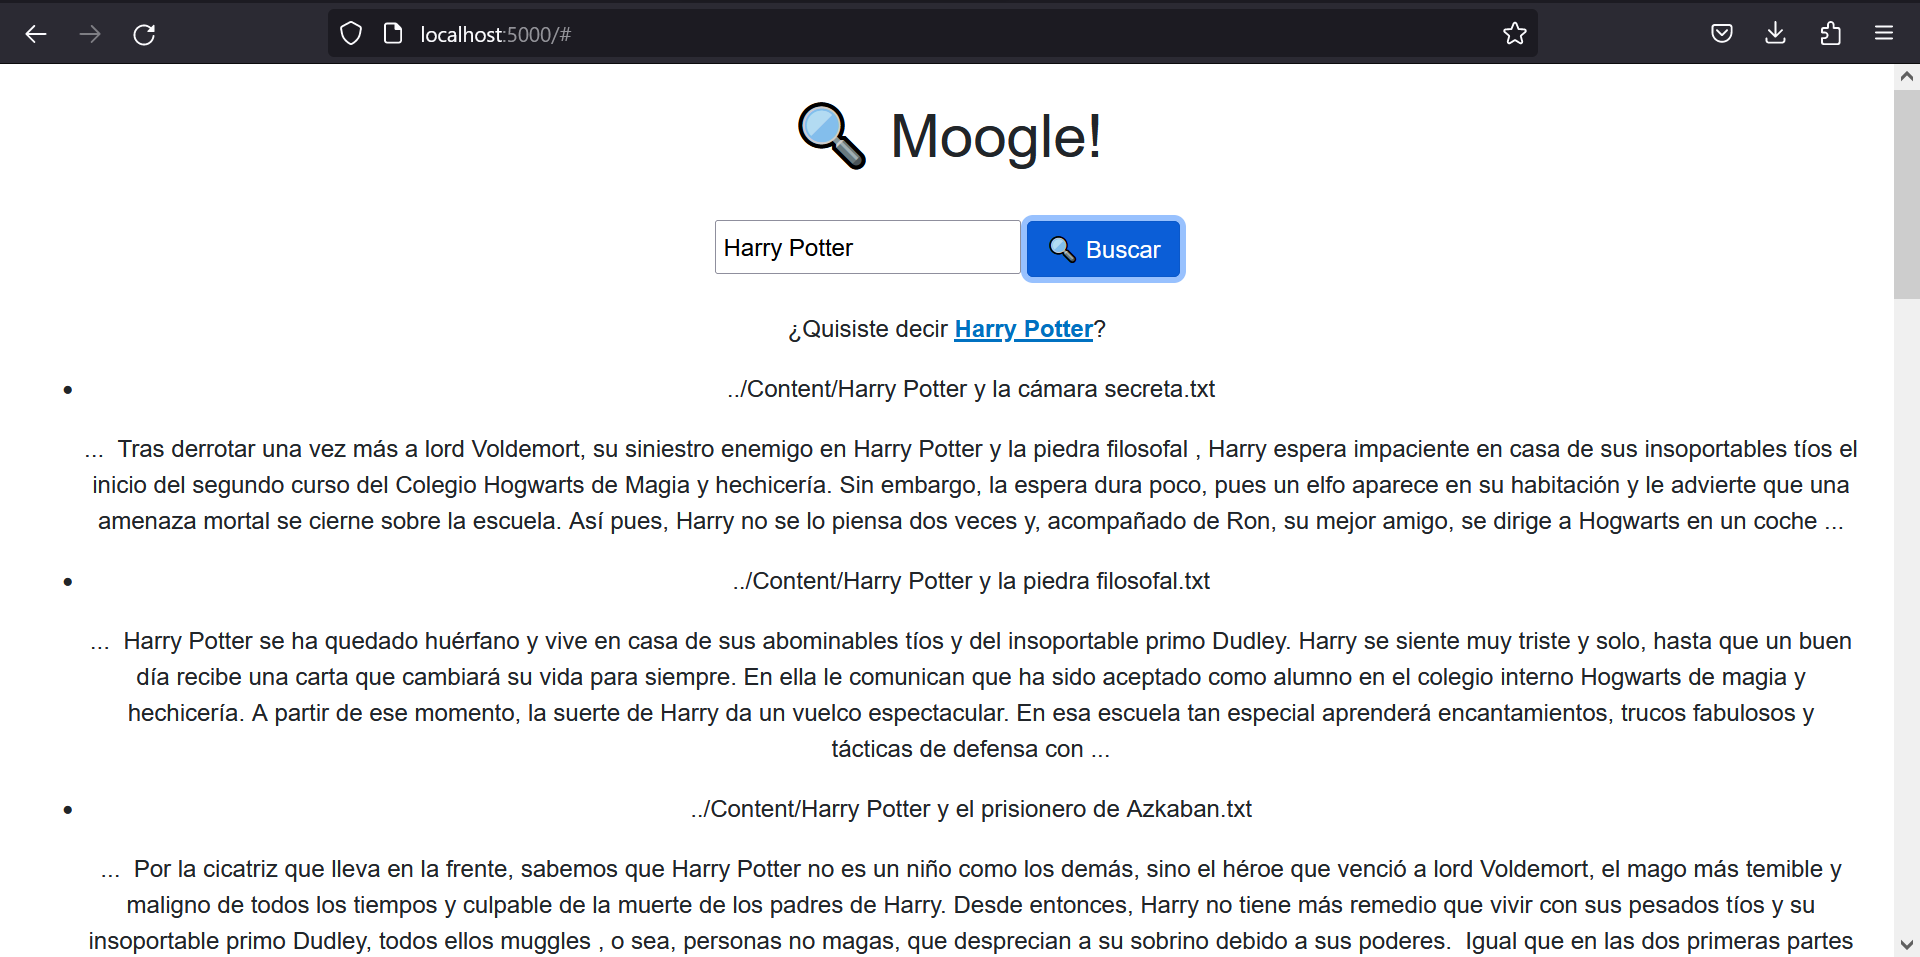
\includegraphics[width=10cm]{images/image 1.png}
      \end{center}
    
\end{frame}

\begin{frame}{\textcolor{cyan}{Resultados}}
    \begin{center}
        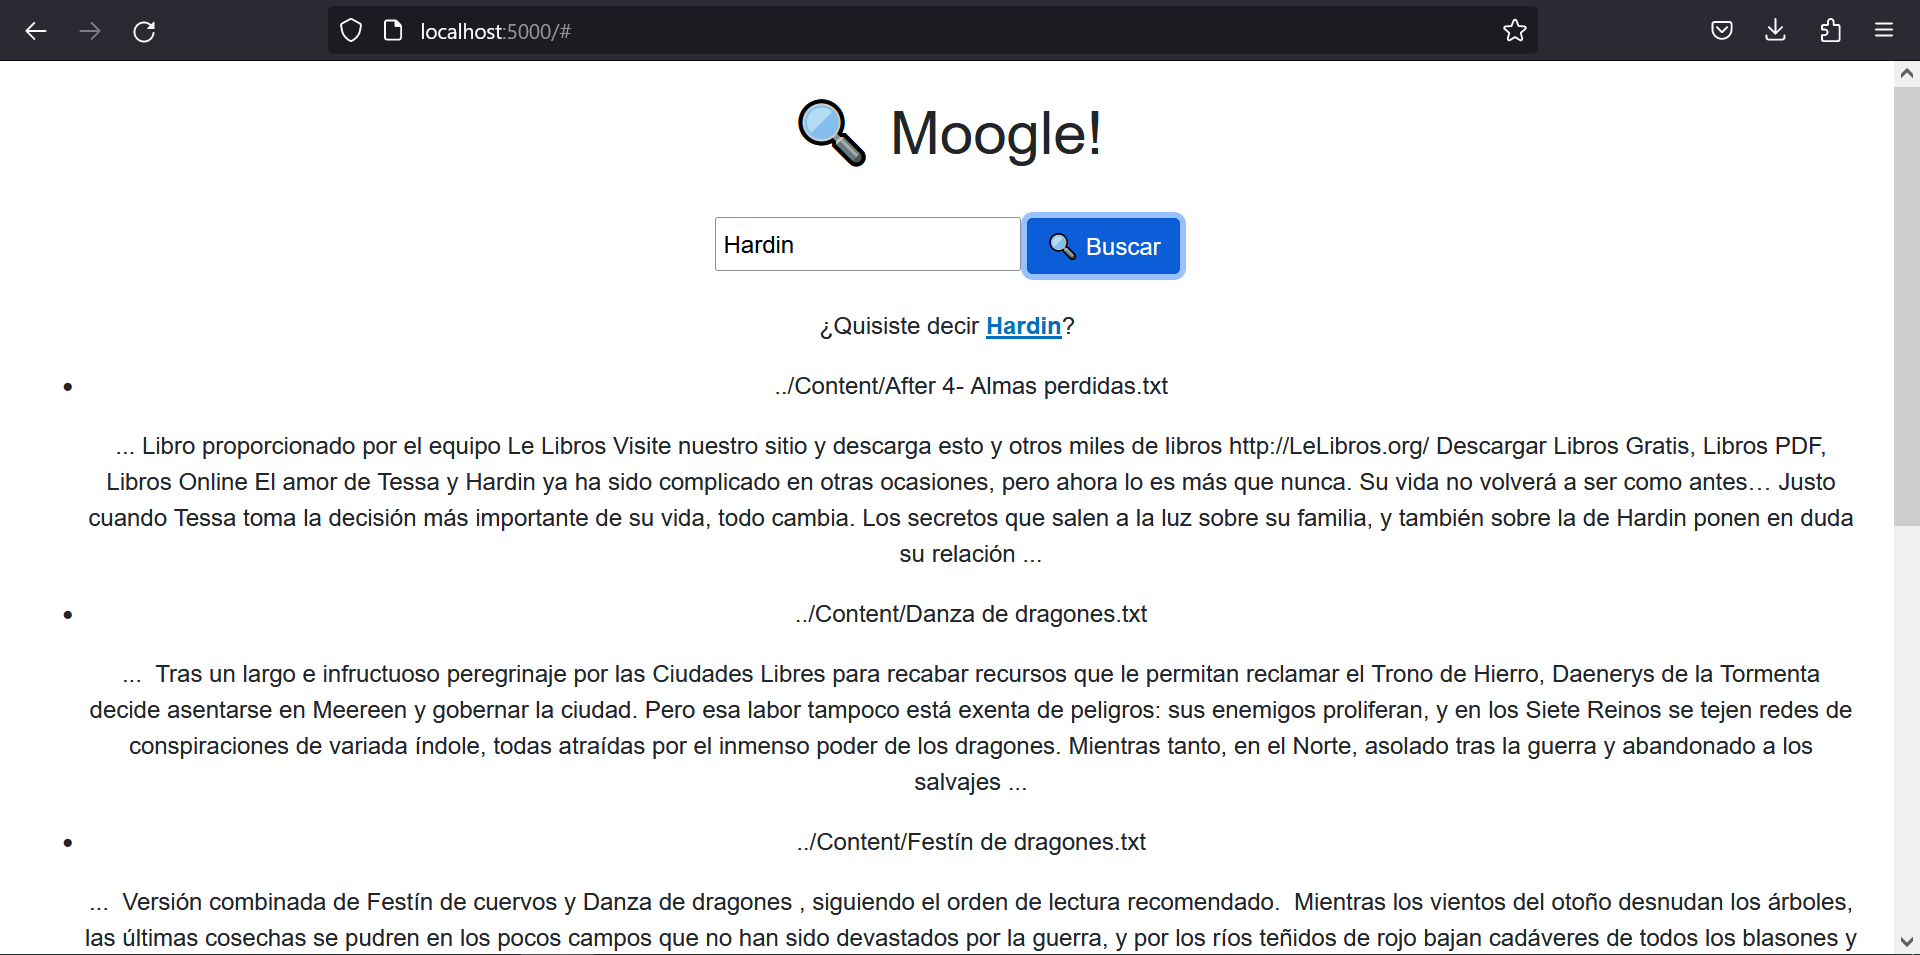
\includegraphics[width=10cm]{images/image 2.png}
      \end{center}
    
\end{frame}

\begin{frame}{\textcolor{cyan}{Resultados}}
    \begin{center}
        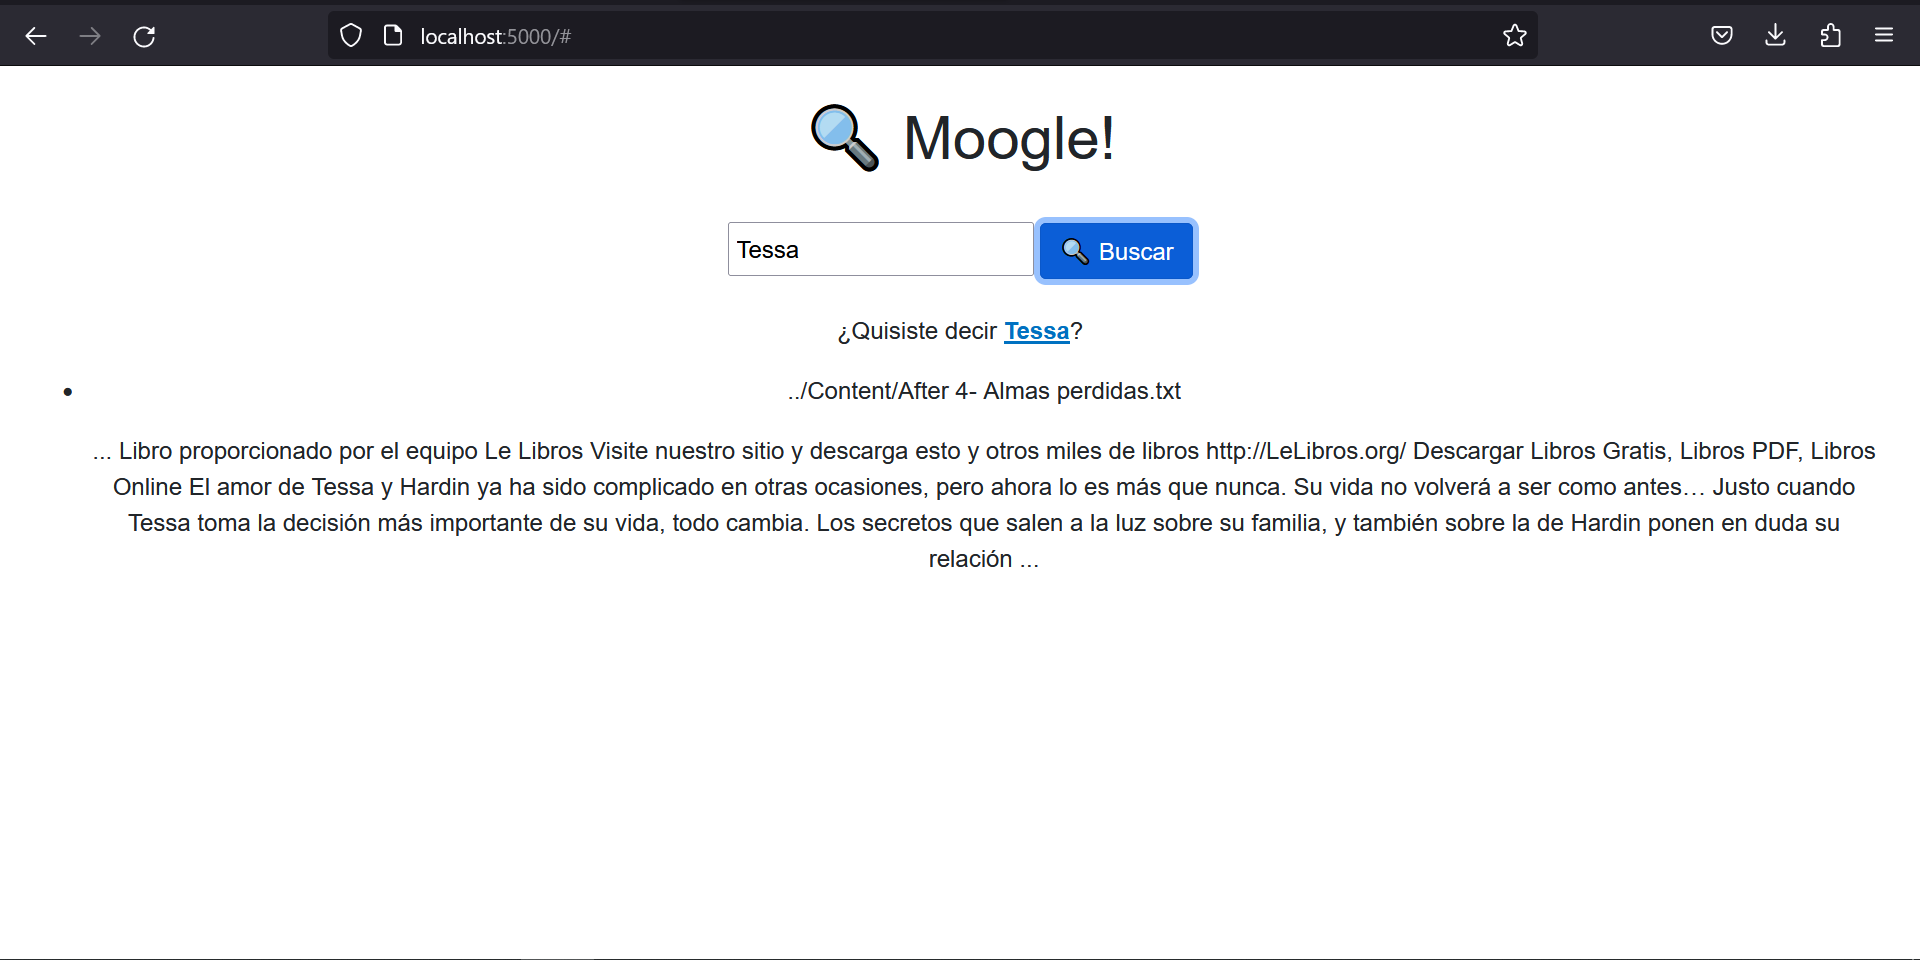
\includegraphics[width=10cm]{images/image 3.png}
      \end{center}
    
\end{frame}

\begin{frame}{\textcolor{cyan}{Resultados}}
    \begin{center}
        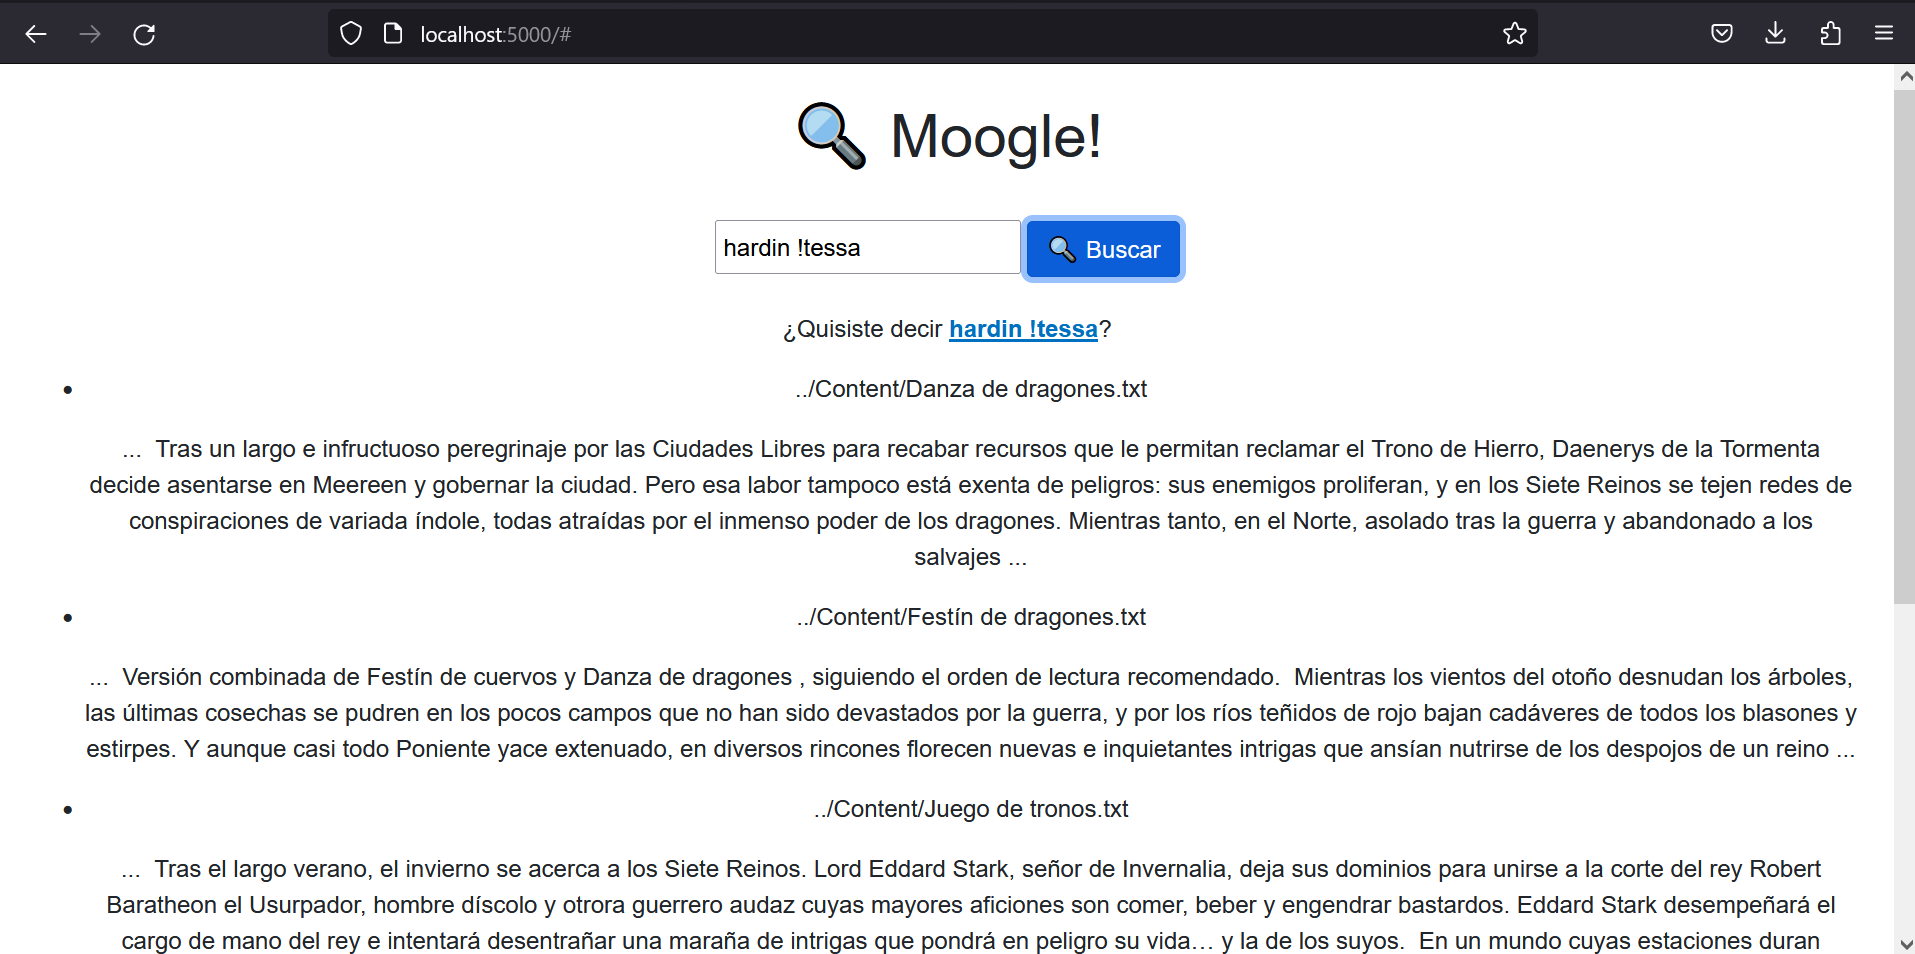
\includegraphics[width=10cm]{images/image 4.png}
      \end{center}
    
\end{frame}

\begin{frame}{\textcolor{cyan}{Resultados}}
    \begin{center}
        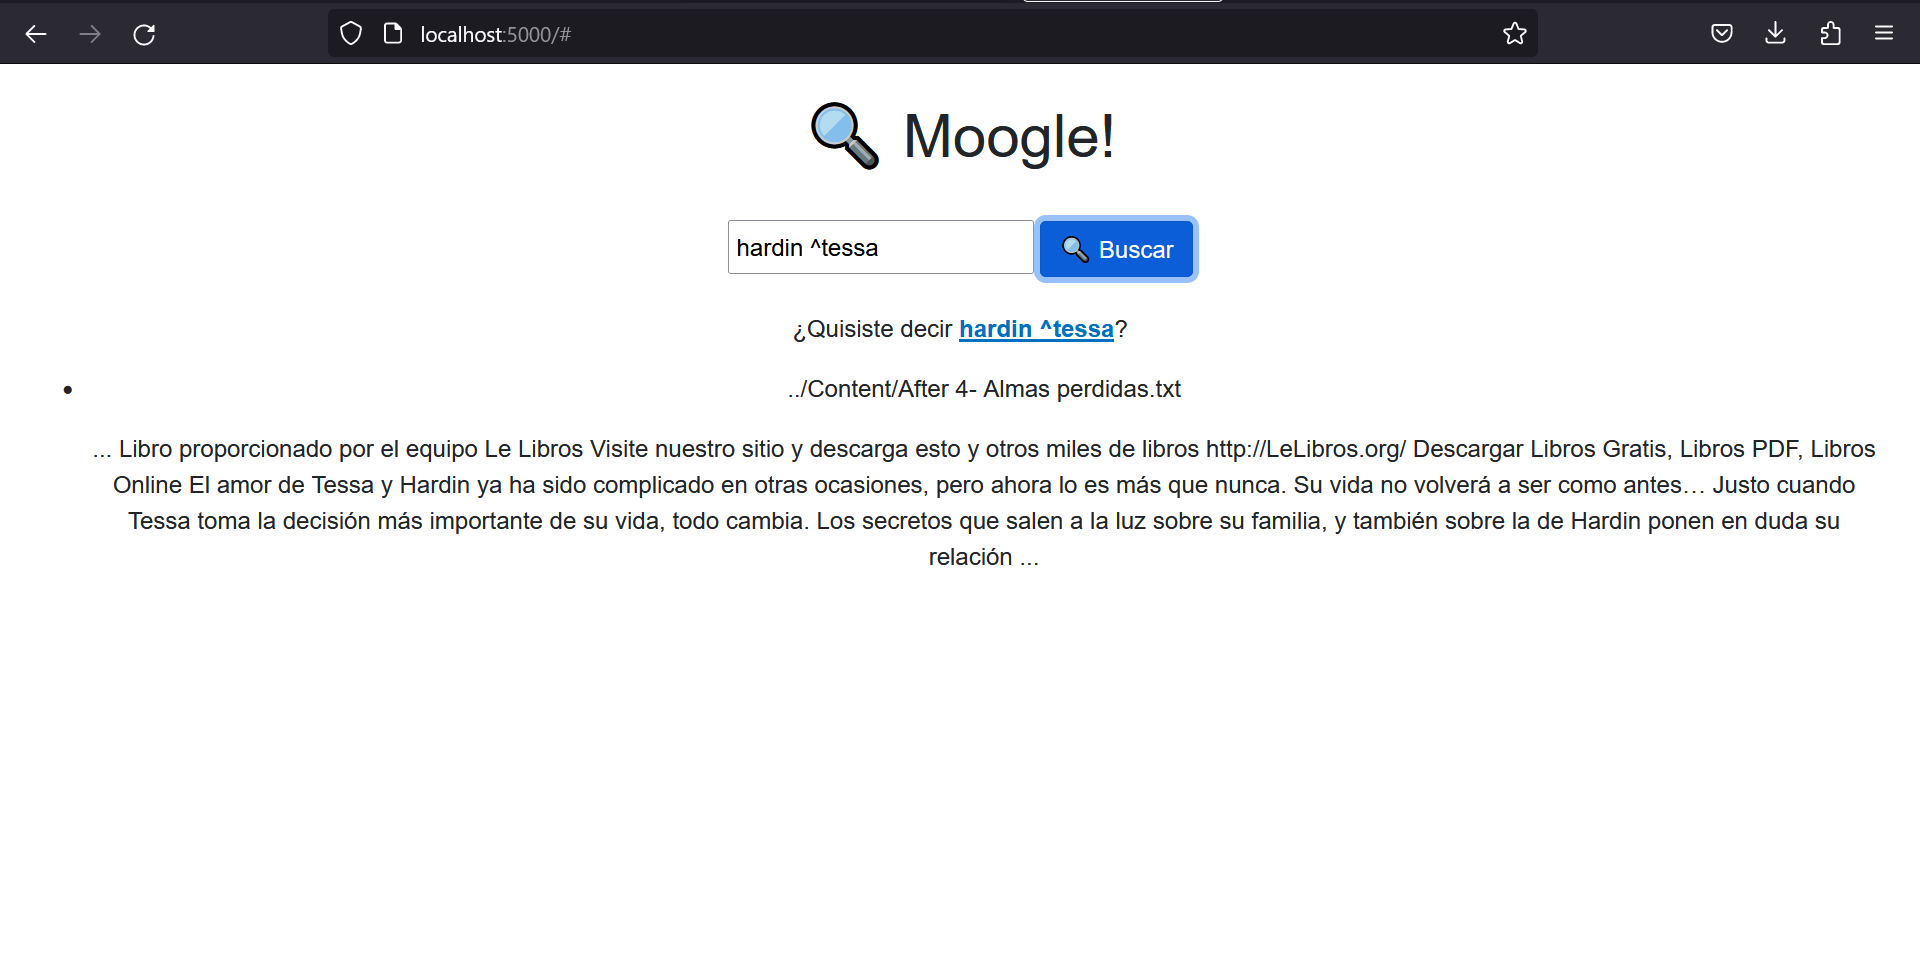
\includegraphics[width=10cm]{images/image 5.png}
      \end{center}
    
\end{frame}

\begin{frame}{\textcolor{cyan}{Resultados}}
    \begin{center}
        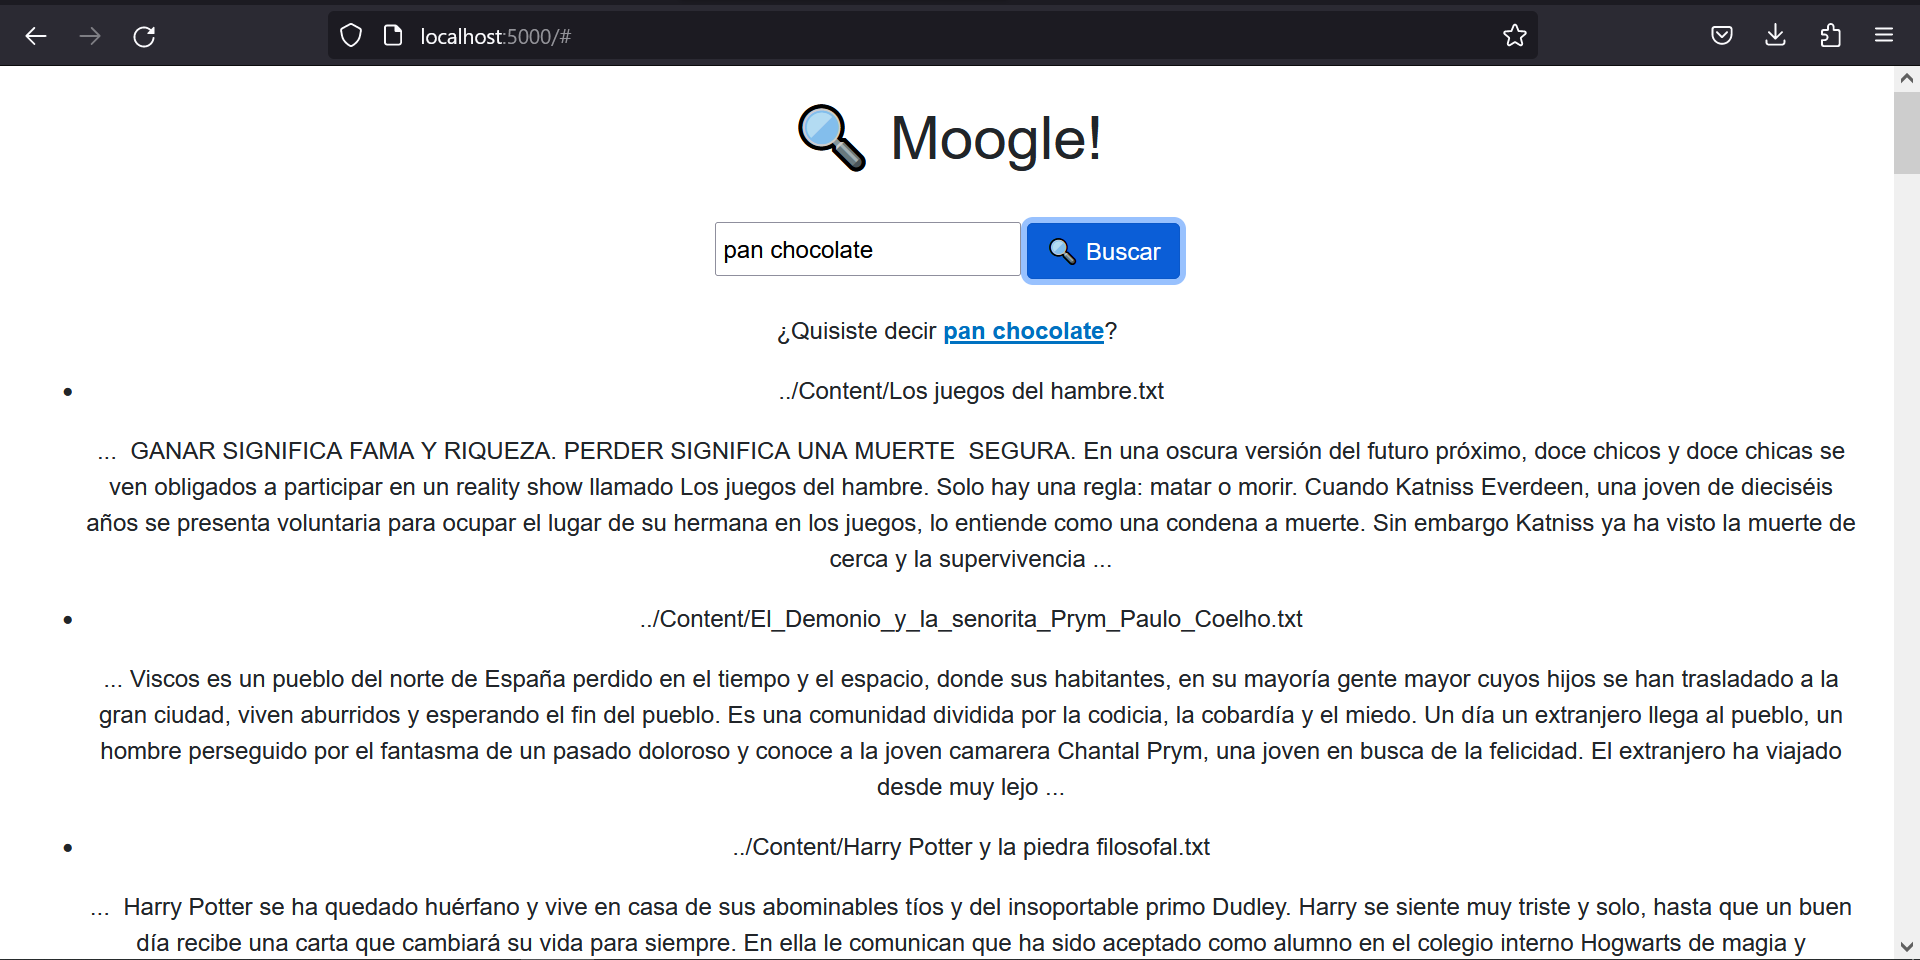
\includegraphics[width=10cm]{images/image 6.png}
      \end{center}
    
\end{frame}

\begin{frame}{\textcolor{cyan}{Resultados}}
    \begin{center}
        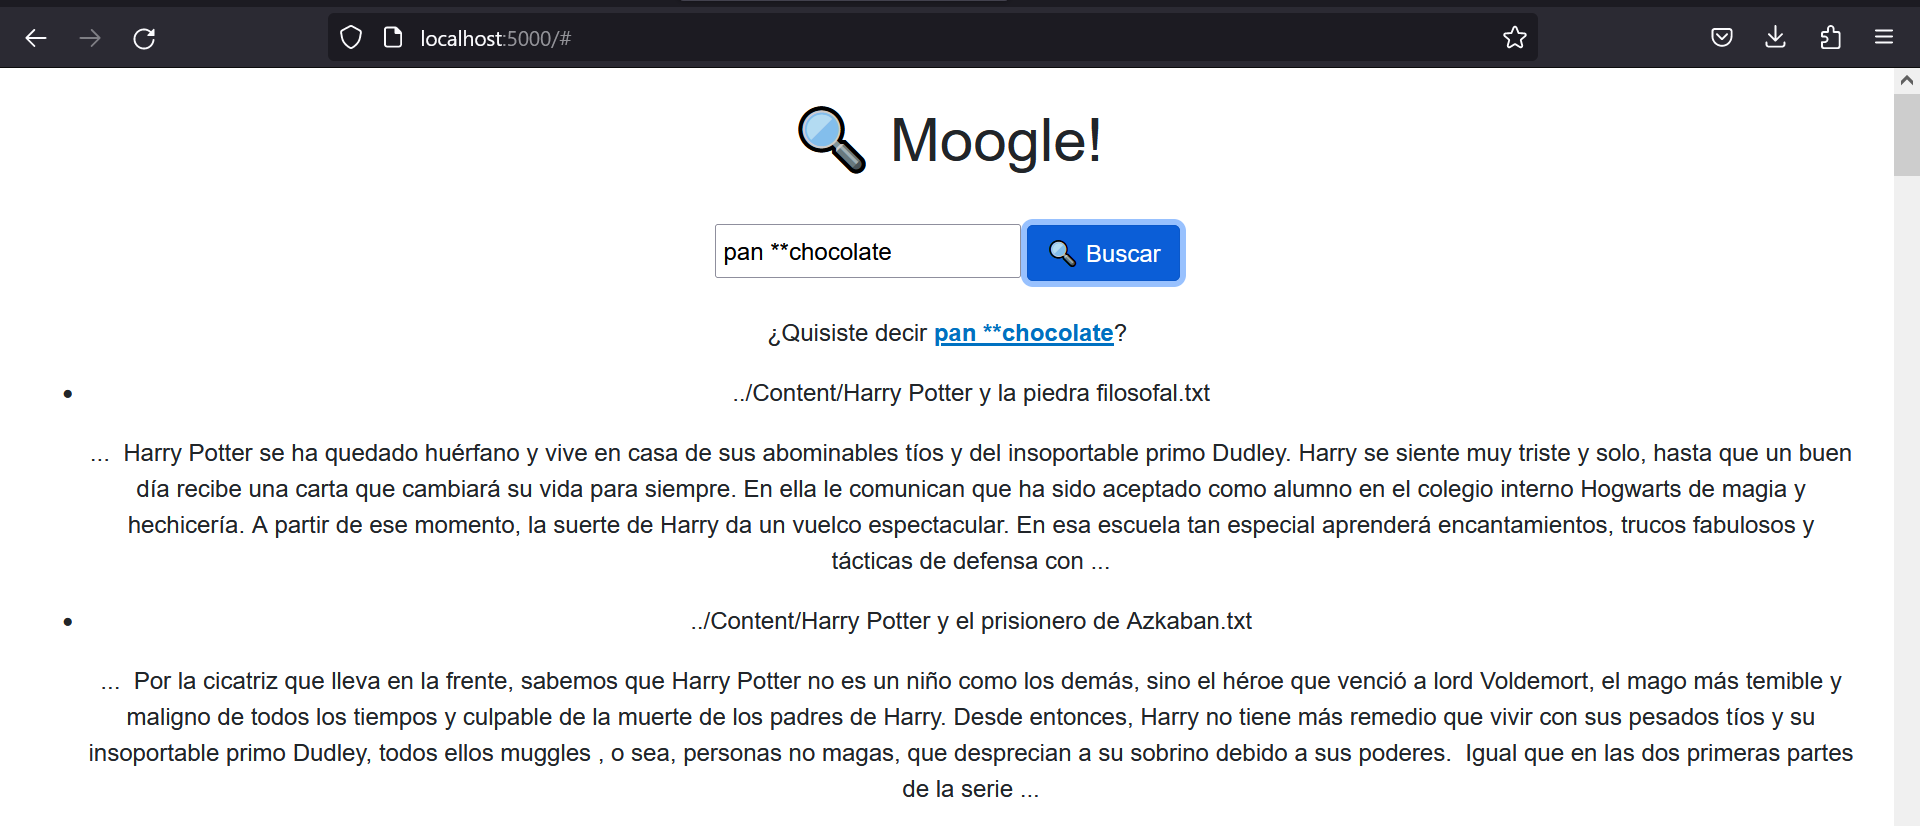
\includegraphics[width=10cm]{images/image 7.png}
      \end{center}
    
\end{frame}
\end{document}